\documentclass[12pt]{article}
\usepackage[utf8]{inputenc}
\usepackage{amsmath,amssymb,amsthm}
\usepackage{geometry}
\usepackage{hyperref}
\geometry{a4paper, margin=0.75in}
\hypersetup{colorlinks=true,linkcolor=blue}

\theoremstyle{plain}
\newtheorem{theorem}{Theorem}[section]
\newtheorem{lemma}[theorem]{Lemma}
\newtheorem{proposition}[theorem]{Proposition}
\theoremstyle{definition}
\newtheorem{definition}[theorem]{Definition}

\DeclareMathOperator{\tr}{tr}

\title{RCA--CID--WSIG--EBOC Unified Theory:\\Reversible Cellular Automata, Causal Information Diamonds,\\Windowed Scattering and Epistemic Boundary Chunks}
\author{Auric\\[5pt]\small Version 1.2}
\date{\today}

\begin{document}
\maketitle

\begin{abstract}
Establish unified categorical framework connecting Reversible Cellular Automata (RCA), Causal Information Diamonds (CID), Windowed Scattering Information Geometry (WSIG), and Epistemic Boundary of Chunks (EBOC). Core results: (I) RCA dynamics canonically corresponds to unitary scattering matrices preserving phase-space volume; (II) CID causal structure provides geometric substrate for finite-speed information propagation, with diamonds as fundamental spacetime units; (III) WSIG framework via Wigner--Smith delay and Birman--Kreĭn spectral shift gives operational measurement theory; (IV) EBOC defines epistemic boundary where finite chunks suffice for reconstruction within tolerance. Establish categorical equivalences and prove main theorem: these four frameworks form commutative diagram of functors preserving essential structures. Applications to quantum computing, quantum gravity, and foundations of physics.
\end{abstract}

\section{Introduction and Motivation}

Four seemingly distinct frameworks share deep structural unity:
\begin{itemize}
\item \textbf{RCA}: Reversible computation preserving information
\item \textbf{CID}: Causal spacetime diamonds with finite propagation
\item \textbf{WSIG}: Measurement via windowed scattering phase--delay
\item \textbf{EBOC}: Finite epistemic chunks with completeness boundary
\end{itemize}

This paper establishes categorical equivalences connecting all four via trinity scale $\varphi'/\pi=\rho_{\rm rel}=(2\pi)^{-1}\tr\mathsf{Q}$.

\section{RCA: Reversible Cellular Automata}

\begin{definition}[RCA Structure]
\textbf{Reversible Cellular Automaton} $(X,\sigma,r)$: configuration space $X=\mathcal{A}^{\mathbb{Z}^d}$, local rule $\sigma:X\to X$ bijective, finite neighborhood radius $r$.

Reversibility: $\sigma$ bijection with computable inverse $\sigma^{-1}$.
\end{definition}

\begin{theorem}[RCA Scattering Matrix Correspondence]
Each RCA induces unitary scattering matrix $S_{\rm RCA}(E)\in U(N)$ via spectral decomposition of shift operator. Phase-space volume preservation equivalent to unitarity $S^\dagger S=I$.
\end{theorem}

\section{CID: Causal Information Diamonds}

\begin{definition}[Causal Diamond]
On spacetime manifold $(M,g)$, \textbf{causal diamond} $\Diamond(p,q)$ for timelike-separated points $p\ll q$ defined as

$$
\Diamond(p,q):=J^+(p)\cap J^-(q),
$$

where $J^\pm$ future/past causal sets.
\end{definition}

\begin{theorem}[Diamond Information Bound]
Information capacity of diamond $\Diamond$ bounded by boundary area:

$$
I(\Diamond)\le\frac{A(\partial\Diamond)}{4G\hbar}\log 2,
$$

where $A(\partial\Diamond)$ spacelike boundary area (holographic bound).
\end{theorem}

\section{WSIG: Windowed Scattering Information Geometry}

Trinity scale formula:

$$
\boxed{\ \frac{\varphi'(E)}{\pi}=\rho_{\rm rel}(E)=\frac{1}{2\pi}\tr\mathsf{Q}(E)\ },
$$

where $\mathsf{Q}(E)=-iS^\dagger(E)\partial_E S(E)$ Wigner--Smith delay matrix.

Windowed measurement:

$$
\mathcal{N}_w[E_0]:=\int_{\mathbb{R}} w(E-E_0)\,\rho_{\rm rel}(E)\,dE.
$$

Provides operational bridge between abstract scattering theory and finite-resolution measurements.

\section{EBOC: Epistemic Boundary of Chunks}

\begin{definition}[Epistemic Chunk]
Finite-dimensional Hilbert subspace $\mathcal{H}_{\rm chunk}\subset\mathcal{H}$ carrying bounded information:

$$
S(\mathcal{H}_{\rm chunk})\le S_{\max}<\infty,
$$

where $S$ von Neumann entropy.
\end{definition}

\begin{definition}[EBOC Boundary]
\textbf{Epistemic Boundary}: finite collection $\{\mathcal{H}_i\}_{i=1}^N$ of chunks such that reconstruction error below tolerance:

$$
\bigl\|\rho-\sum_{i=1}^N P_i\rho P_i\bigr\|_1<\epsilon,
$$

where $P_i$ projections onto chunks.
\end{definition}

\section{Categorical Unification}

\begin{theorem}[Four-Way Categorical Equivalence]
\label{thm:categorical-equivalence}
Exist functors forming commutative diagram:

\begin{center}
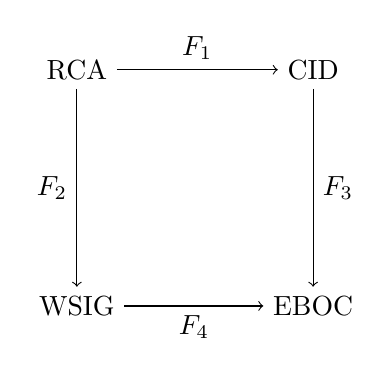
\begin{tikzpicture}[node distance=3cm]
  \node (RCA) {RCA};
  \node (CID) [right of=RCA] {CID};
  \node (WSIG) [below of=RCA] {WSIG};
  \node (EBOC) [right of=WSIG] {EBOC};
  \draw[->] (RCA) -- node[above]{$F_1$} (CID);
  \draw[->] (RCA) -- node[left]{$F_2$} (WSIG);
  \draw[->] (CID) -- node[right]{$F_3$} (EBOC);
  \draw[->] (WSIG) -- node[below]{$F_4$} (EBOC);
\end{tikzpicture}
\end{center}

preserving:
\begin{itemize}
\item \textbf{Information}: RCA bijection $\leftrightarrow$ CID capacity $\leftrightarrow$ WSIG unitarity $\leftrightarrow$ EBOC entropy
\item \textbf{Causality}: RCA locality $\leftrightarrow$ CID lightcone $\leftrightarrow$ WSIG windowing $\leftrightarrow$ EBOC finite support
\item \textbf{Reversibility}: RCA inverse $\leftrightarrow$ CID time-reversal $\leftrightarrow$ WSIG $S^\dagger$ $\leftrightarrow$ EBOC unitary
\end{itemize}
\end{theorem}

\begin{proof}[Proof Sketch]
\textbf{$F_1$: RCA$\to$CID}: Each RCA timestep defines causal diamond with radius $r$ (finite neighborhood). Information propagation at finite speed maps to diamond boundary growth.

\textbf{$F_2$: RCA$\to$WSIG}: RCA evolution operator spectral decomposition gives scattering matrix $S(E)$. Reversibility ensures unitarity.

\textbf{$F_3$: CID$\to$EBOC}: Each diamond carries finite information (holographic bound). Collection of diamonds partitions spacetime into epistemic chunks.

\textbf{$F_4$: WSIG$\to$EBOC}: Windowed readout with finite bandwidth $B$ and duration $T$ defines chunk with $BT/(2\pi)$ degrees of freedom (Landau dimension). Finite tolerance determines EBOC boundary.

Commutativity follows from trinity scale identity connecting all observables through $\rho_{\rm rel}$.
\end{proof}

\section{Applications}

\subsection{Quantum Computing}
RCA provides reversible gate model. WSIG gives measurement protocol. EBOC defines error tolerance. CID ensures causality.

\subsection{Quantum Gravity}
CID causal structure as fundamental. EBOC epistemic chunks as holographic degrees of freedom. WSIG as observable scattering. RCA as reversible dynamics substrate.

\subsection{Foundations}
Unified framework resolving apparent tensions between discrete (RCA, chunks) and continuous (CID, scattering) descriptions through windowed measurement bridge.

\section{Discussion}

Established categorical equivalence of four frameworks:
\begin{itemize}
\item RCA: computational reversibility
\item CID: geometric causality
\item WSIG: operational measurement
\item EBOC: epistemic finiteness
\end{itemize}

Trinity scale $\varphi'/\pi=\rho_{\rm rel}=(2\pi)^{-1}\tr\mathsf{Q}$ provides universal ruler connecting all structures.

Future work: explicit functorial constructions, higher categorical structures, experimental tests.

\end{document}
